\documentclass{article}
\usepackage[utf8]{inputenc}
\usepackage{amsmath}
\usepackage{amssymb}
\usepackage{graphicx}
\usepackage{bm}
\usepackage{hyperref}
\usepackage[margin=0.8in]{geometry}

\title{Computational Neuroscience - Homework Module 2}
\author{Sepehr SAEEDPOUR}
\date{May 2025}

\begin{document}

\maketitle

\section{Covariance and Correlation}

\subsection{Variance of firing rates}
We need to show that $\text{Var}(r_1) = \frac{1}{N-1} \|x\|^2$.

The variance of $r_1$ is defined as:
\begin{align}
\text{Var}(r_1) &= \frac{1}{N-1}\sum_{i=1}^{N}(r_{1,i} - \bar{r}_1)^2
\end{align}

% Looking at our vector $x$:
% \begin{align}
% x &= 
% \begin{pmatrix}
% r_{1,1} - \bar{r}_1 \\
% r_{1,2} - \bar{r}_1 \\
% r_{1,3} - \bar{r}_1 \\
% \vdots \\
% r_{1,N} - \bar{r}_1
% \end{pmatrix}
% \end{align}

The squared norm of $x$ is:
\begin{align}
\|x\|^2 &= (r_{1,1} - \bar{r}_1)^2 + (r_{1,2} - \bar{r}_1)^2 + \ldots + (r_{1,N} - \bar{r}_1)^2 \\
&= \sum_{i=1}^{N}(r_{1,i} - \bar{r}_1)^2
\end{align}

Therefore:
\begin{align}
\text{Var}(r_1) &= \frac{1}{N-1}\sum_{i=1}^{N}(r_{1,i} - \bar{r}_1)^2 \\
&= \frac{1}{N-1}\|x\|^2
\end{align}

Please note that when we estimate variance from a sample using the sample mean, the result tends to underestimate the true population variance (i.e., biased estimator). N-1 as a divisor instead N (Bessel's correction) fixes this by compensating for the loss of one degree of freedom from using the sample mean. This adjustment makes the sample variance an unbiased estimator of the population variance.

\subsection{Cosine of angle between $x$ and $y$}
The cosine of the angle between two vectors $x$ and $y$ is:
\begin{align}
\cos(\theta) = \frac{x \cdot y}{\|x\| \cdot \|y\|}
\end{align}

Let's calculate each component:
\begin{align}
x \cdot y &= \sum_{i=1}^{N}(r_{1,i} - \bar{r}_1)(r_{2,i} - \bar{r}_2) \\
&= (N-1) \cdot \text{Cov}(r_1, r_2)
\end{align}

For the denominator:
\begin{align}
\|x\| \cdot \|y\| &= \sqrt{\sum_{i=1}^{N}(r_{1,i} - \bar{r}_1)^2} \cdot \sqrt{\sum_{i=1}^{N}(r_{2,i} - \bar{r}_2)^2} \\
&= \sqrt{(N-1) \cdot \text{Var}(r_1)} \cdot \sqrt{(N-1) \cdot \text{Var}(r_2)} \\
&= (N-1) \cdot \sqrt{\text{Var}(r_1) \cdot \text{Var}(r_2)}
\end{align}

Therefore:
\begin{align}
\cos(\theta) &= \frac{(N-1) \cdot \text{Cov}(r_1, r_2)}{(N-1) \cdot \sqrt{\text{Var}(r_1) \cdot \text{Var}(r_2)}} \\
&= \frac{\text{Cov}(r_1, r_2)}{\sqrt{\text{Var}(r_1) \cdot \text{Var}(r_2)}} \\
&= \text{corr}(r_1, r_2)
\end{align}

Thus, the cosine of the angle between $x$ and $y$ is exactly the correlation coefficient between $r_1$ and $r_2$.

\subsection{Maximum and minimum values of correlation coefficient}
The correlation coefficient (and therefore the cosine of the angle) ranges from $-1$ to $1$:
\begin{itemize}
\item Maximum value: $1$ (when the vectors are perfectly aligned, i.e., angle = $0^\circ$)
\item Minimum value: $-1$ (when the vectors point in opposite directions, i.e., angle = $180^\circ$)
\end{itemize}

The correlation is $1$ when the two variables are perfectly positively linearly related, and $-1$ when they are perfectly negatively linearly related. The correlation is $0$ when there is no linear relationship between the variables.

\subsection{Meaning of "centered"}
Here, we're centering the firing rates by subtracting their respective means ($\bar{r}_1$ and $\bar{r}_2$). In fact, "Centered" refers to subtracting the mean from each data point, moving the mean of the data to zero. This transformation moves the data to be centered around the origin in the coordinate system. It's an important preprocessing step in many statistical analyses (e.g., PCA)

\section{Ridge Regression – Closed-Form Solution}

\subsection{Penalizing complex models}
The term $\lambda\|w\|^2$ penalizes complex models by adding a cost proportional to the squared magnitude of the weight vector. This regularization:

\begin{itemize}
\item Discourages large weights, which often correspond to overfitting
\item Makes the model less sensitive to noise in the training data
\item Promotes smoother, more generalizable models
\item Stabilizes the solution when features are highly correlated
\end{itemize}

Intuitively, large weights amplify the influence of individual features, potentially allowing the model to fit noise rather than the underlying pattern. By keeping the weights small, the model becomes more robust.

\subsection{Solution for $\lambda = 0$ (no regularization)}
Starting with the error function:
\begin{align}
E(w) &= \|y - Xw\|^2
\end{align}

Expanding:
\begin{align}
E(w) &= (y - Xw)^T(y - Xw) \\
&= y^Ty - y^TXw - w^TX^Ty + w^TX^TXw \\
&= y^Ty - 2w^TX^Ty + w^TX^TXw \quad \text{(since $y^TXw$ is a scalar)}
\end{align}

To find the minimum, we take the derivative with respect to $w$ and set it to zero:
\begin{align}
\frac{\partial E}{\partial w} &= -2X^Ty + 2X^TXw = 0
\end{align}

Solving for $w$:
\begin{align}
X^TXw &= X^Ty \\
w &= (X^TX)^{-1}X^Ty
\end{align}

This is the normal equation solution, where $(X^TX)^{-1}X^T$ is the pseudo-inverse of $X$.

\subsection{Solution for $\lambda > 0$ (with regularization)}
With regularization:
\begin{align}
E(w) &= \|y - Xw\|^2 + \lambda\|w\|^2 \\
&= (y - Xw)^T(y - Xw) + \lambda w^Tw \\
&= y^Ty - 2w^TX^Ty + w^TX^TXw + \lambda w^Tw \\
&= y^Ty - 2w^TX^Ty + w^T(X^TX + \lambda I)w
\end{align}

Taking the derivative and setting it to zero:
\begin{align}
\frac{\partial E}{\partial w} &= -2X^Ty + 2(X^TX + \lambda I)w = 0
\end{align}

Solving for $w$:
\begin{align}
(X^TX + \lambda I)w &= X^Ty \\
w &= (X^TX + \lambda I)^{-1}X^Ty
\end{align}

\subsection{Purpose of adding $\lambda I$ to $X^TX$}
Adding $\lambda I$ to $X^TX$ addresses potential numerical instability and invertibility issues. Specifically:

\begin{itemize}
\item It ensures that $X^TX + \lambda I$ is always invertible, even when $X^TX$ is singular or near-singular
\item It provides a solution when features are highly correlated (multicollinearity)
\item It improves the condition number of the matrix, making the solution more stable
\item It enables a solution even when there are more features than data points ($d > n$)
\end{itemize}

Without regularization, $X^TX$ might be rank-deficient (i.e., some eigenvalues are zero), making inversion impossible. Since $\lambda I$ has all eigenvalues equal to $\lambda > 0$, adding it to $X^TX$ ensures all eigenvalues of the resulting matrix are positive, making it positive definite and therefore invertible.

\subsection{Optimal value for $\lambda$}
There is no single "optimal" value for $\lambda$ that works for all problems. The optimal $\lambda$ is typically determined through cross-validation:

\begin{enumerate}
\item Split the data into training and validation sets
\item Fit the model on the training set with different values of $\lambda$
\item Evaluate the model's performance on the validation set for each $\lambda$
\item Choose the $\lambda$ that minimizes the validation error
\end{enumerate}

This process helps balance the bias-variance tradeoff: too small $\lambda$ may lead to overfitting, while too large $\lambda$ may cause underfitting.

\section{Bayes' theorem}

\subsection{Calculating $p(r)$}
We can calculate $p(r)$ using the law of total probability:
\begin{align}
p(r) &= p(r|\leftarrow)p(\leftarrow) + p(r|\rightarrow)p(\rightarrow)
\end{align}

Given that $p(r|s)$ follows a Gaussian distribution for each stimulus $s$:
\begin{align}
p(r|s) &= \frac{1}{\sqrt{2\pi\sigma^2}} \exp\left(-\frac{(r - \mu_s)^2}{2\sigma^2}\right)
\end{align}

Therefore:
\begin{align}
p(r) &= p(\leftarrow) \cdot \frac{1}{\sqrt{2\pi\sigma^2}} \exp\left(-\frac{(r - \mu_\leftarrow)^2}{2\sigma^2}\right) + p(\rightarrow) \cdot \frac{1}{\sqrt{2\pi\sigma^2}} \exp\left(-\frac{(r - \mu_\rightarrow)^2}{2\sigma^2}\right) \\
&= \frac{1}{\sqrt{2\pi\sigma^2}} \left[ p(\leftarrow) \exp\left(-\frac{(r - \mu_\leftarrow)^2}{2\sigma^2}\right) + p(\rightarrow) \exp\left(-\frac{(r - \mu_\rightarrow)^2}{2\sigma^2}\right) \right]
\end{align}

This is a mixture of two Gaussians with means $\mu_\leftarrow$ and $\mu_\rightarrow$, standard deviation $\sigma$, and mixing proportions $p(\leftarrow)$ and $p(\rightarrow)$.

Let the standardized separation be
\[
d=\frac{\lvert\mu_{\rightarrow}-\mu_{\leftarrow}\rvert}{\sigma}.
\]
When \(d\lesssim 1\) the two bells overlap so much that the mixture shows just one, slightly broader peak (leaning toward the heavier‐weighted side if the mixing proportions differ).  
For \(1\lesssim d\lesssim 2\) this peak develops a flat top or shoulder.  
Once \(d\gtrsim 2\) (and even larger if one component is much rarer) the curve splits into two distinct peaks; the taller peak lies under the component with the larger mixing weight.


\subsection{Posterior calculation with equal priors}
With $p(\leftarrow) = p(\rightarrow) = 1/2$, the posterior is:
\begin{align}
p(\leftarrow|r) &= \frac{p(r|\leftarrow)p(\leftarrow)}{p(r)} \\
&= \frac{p(r|\leftarrow) \cdot \frac{1}{2}}{p(r|\leftarrow) \cdot \frac{1}{2} + p(r|\rightarrow) \cdot \frac{1}{2}} \\
&= \frac{p(r|\leftarrow)}{p(r|\leftarrow) + p(r|\rightarrow)} \\
&= \frac{\exp\left(-\frac{(r - \mu_\leftarrow)^2}{2\sigma^2}\right)}{\exp\left(-\frac{(r - \mu_\leftarrow)^2}{2\sigma^2}\right) + \exp\left(-\frac{(r - \mu_\rightarrow)^2}{2\sigma^2}\right)} \\
&= \frac{1}{1 + \exp\left(-\frac{(r - \mu_\leftarrow)^2 - (r - \mu_\rightarrow)^2}{2\sigma^2}\right)} \\
&= \frac{1}{1 + \exp\left(-\frac{2r(\mu_\rightarrow - \mu_\leftarrow) + \mu_\leftarrow^2 - \mu_\rightarrow^2}{2\sigma^2}\right)}
\end{align}

Similarly, for $p(\rightarrow|r)$ we get:

\begin{align}
p(\rightarrow|r) &= \frac{1}{1 + \exp\left(-\frac{2r(\mu_\leftarrow - \mu_\rightarrow) + \mu_\rightarrow^2 - \mu_\leftarrow^2}{2\sigma^2}\right)}
\end{align}

The posterior would produce a sigmoid-shaped curve, crossing at the midpoint between $\mu_\leftarrow$ and $\mu_\rightarrow$, where $p(\leftarrow|r) = p(\rightarrow|r) = 0.5$.



\begin{figure}[h]
    \centering
    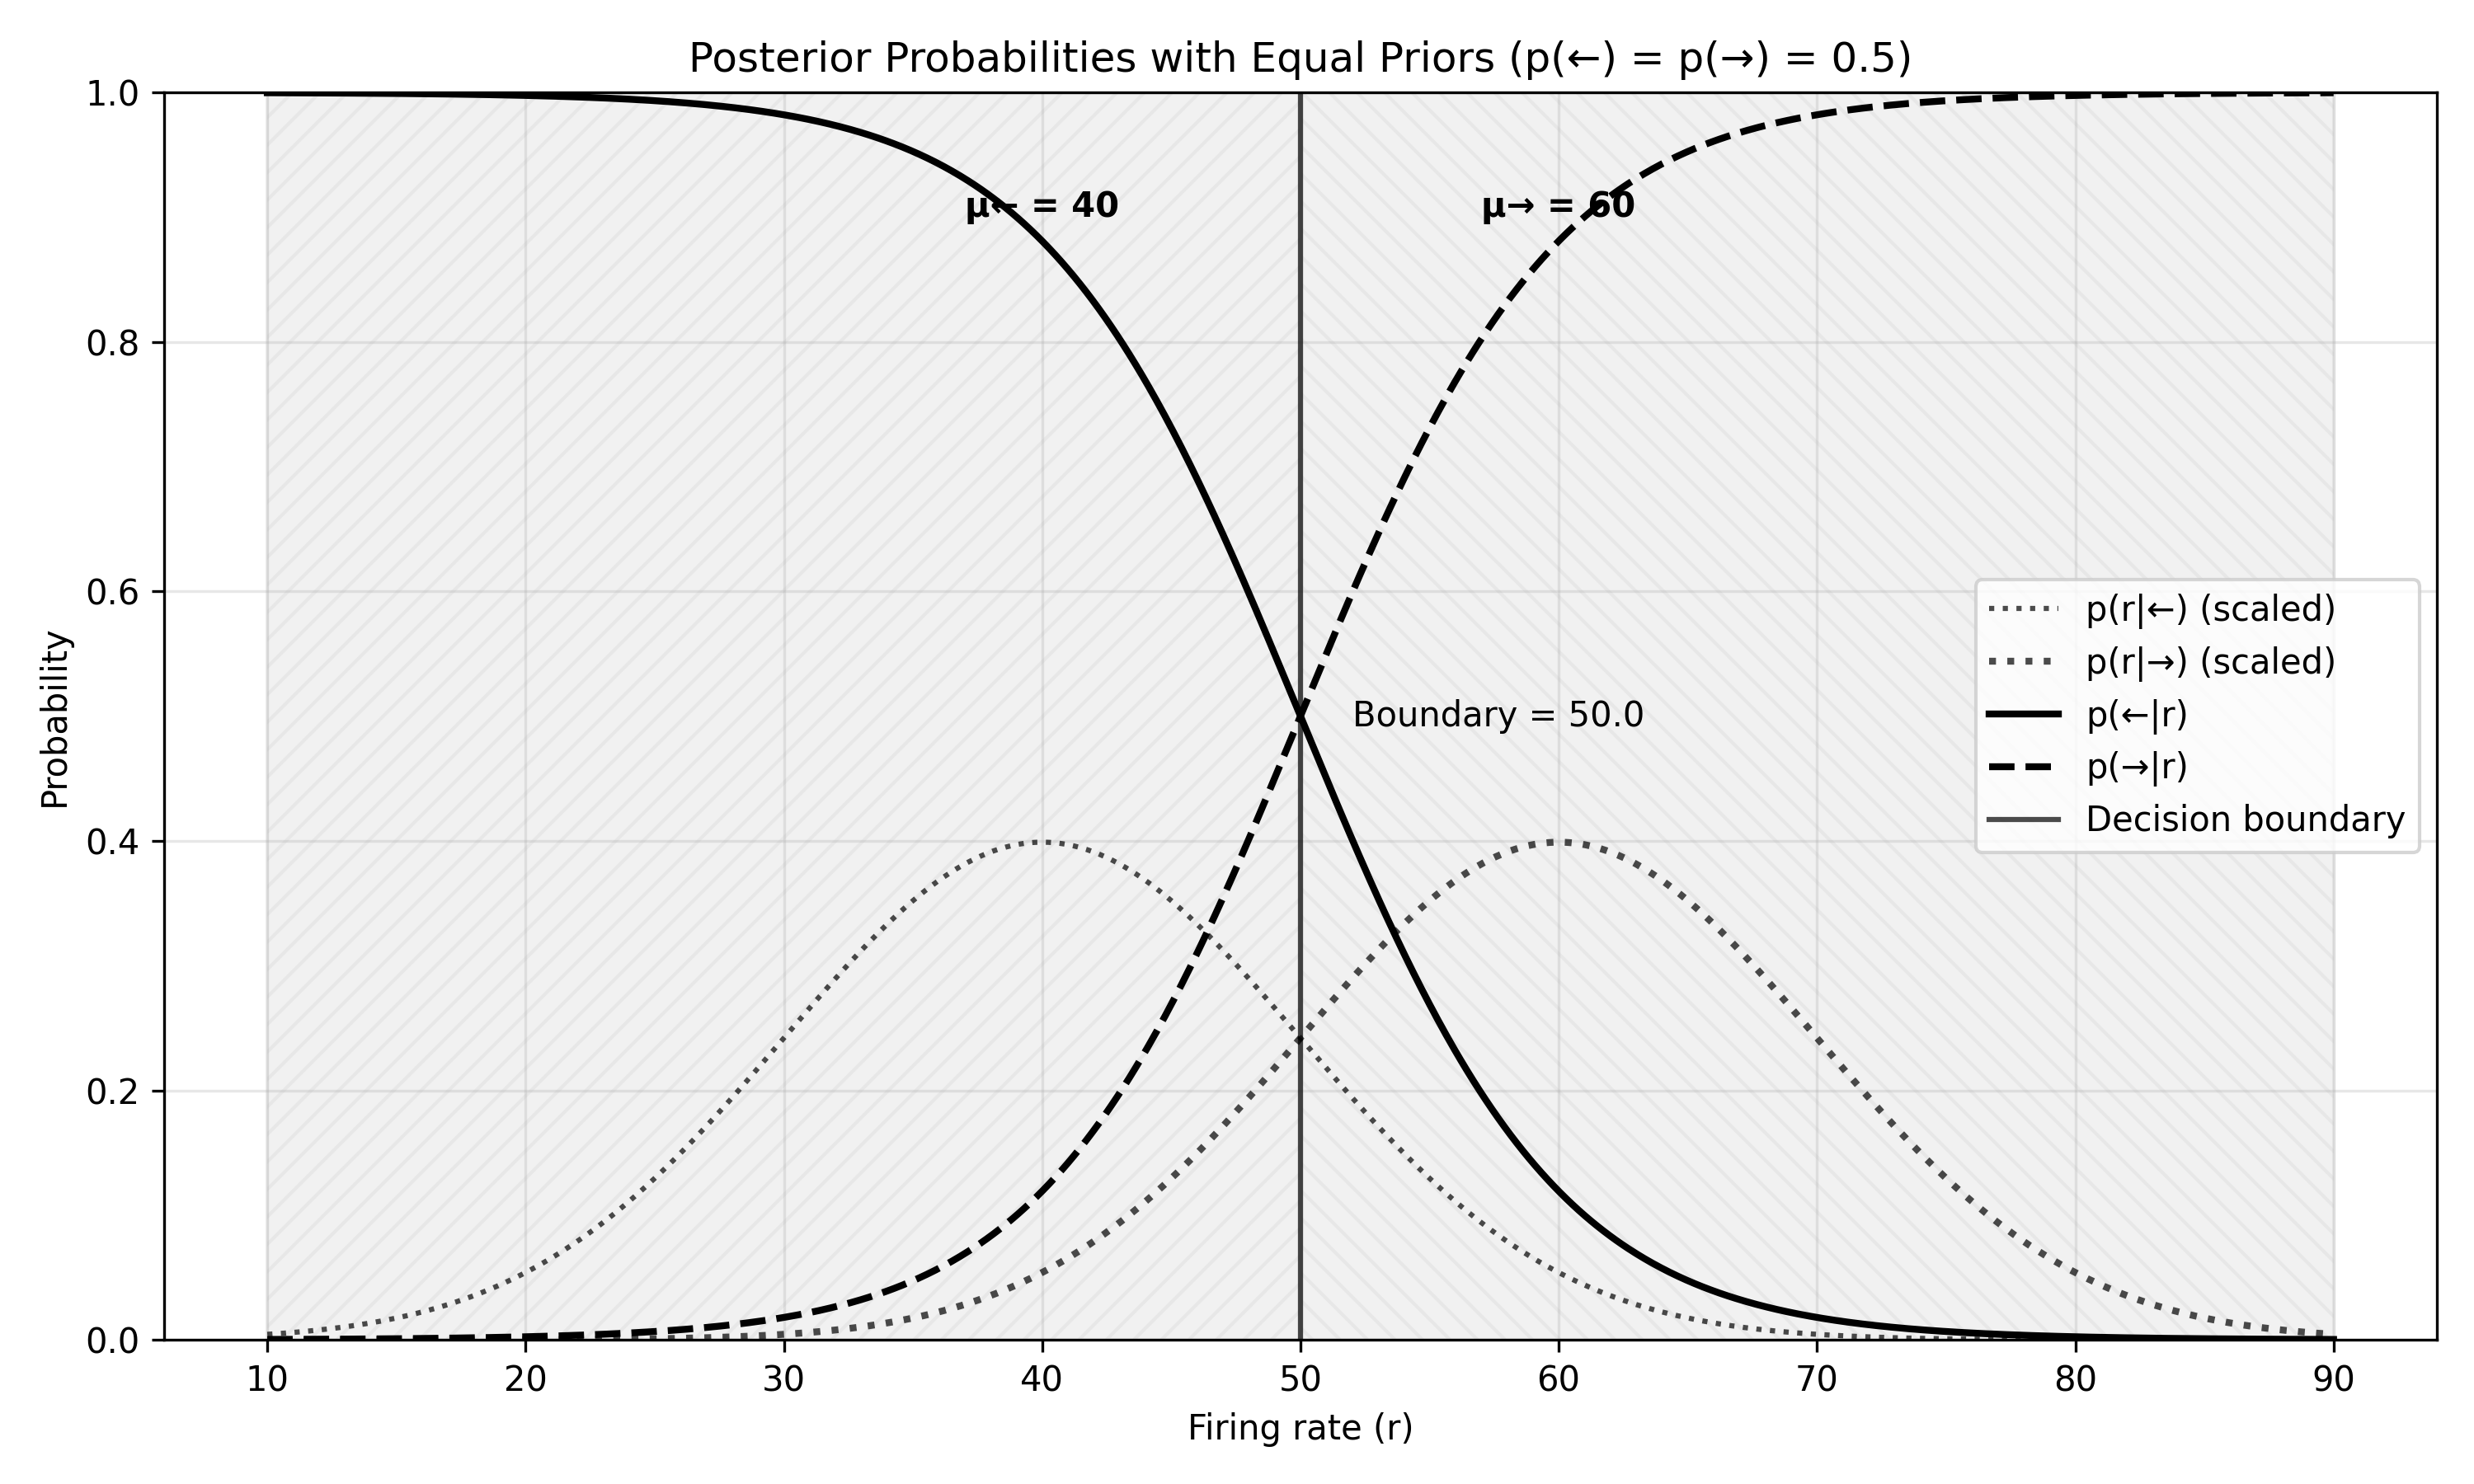
\includegraphics[width=0.8\textwidth]{posterior_equal_priors.png}
    \caption{Posterior probabilities for the equal--prior case,
    \(p(\leftarrow)=p(\rightarrow)=0.5\).
    The solid black curve shows \(p(\leftarrow\mid r)\) and the dashed black curve
    shows \(p(\rightarrow\mid r)\).
    Grey dotted lines depict the (rescaled) likelihoods
    \(p(r\mid\leftarrow)\) and \(p(r\mid\rightarrow)\).
    The two posteriors are complementary sigmoids that intersect at
    \(r=50\), the midpoint between the means
    \(\mu_{\leftarrow}=40\) and \(\mu_{\rightarrow}=60\).
    The vertical line marks this optimal decision boundary.}
    \label{fig:bayes_posterior}
\end{figure}

\pagebreak
% Note that you would need to create the actual image file "bayes_posterior.png" showing these curves. Such a figure would visually demonstrate how the posterior probabilities form sigmoid curves and how the prior probabilities affect the decision boundary.


\subsection{Effect of changing the prior}
When the priors are unequal, the posterior probabilities shift accordingly:

\begin{itemize}
\item When $p(\leftarrow) > p(\rightarrow)$, the sigmoid curve shifts to the right, making leftward motion more likely for a wider range of firing rates
\item When $p(\rightarrow) > p(\leftarrow)$, the curve shifts to the left, favoring rightward motion for more firing rates
\end{itemize}

The crossing point of the posteriors (where $p(\leftarrow|r) = p(\rightarrow|r)$) moves away from the midpoint between the means.


\begin{figure}[h]
    \centering
    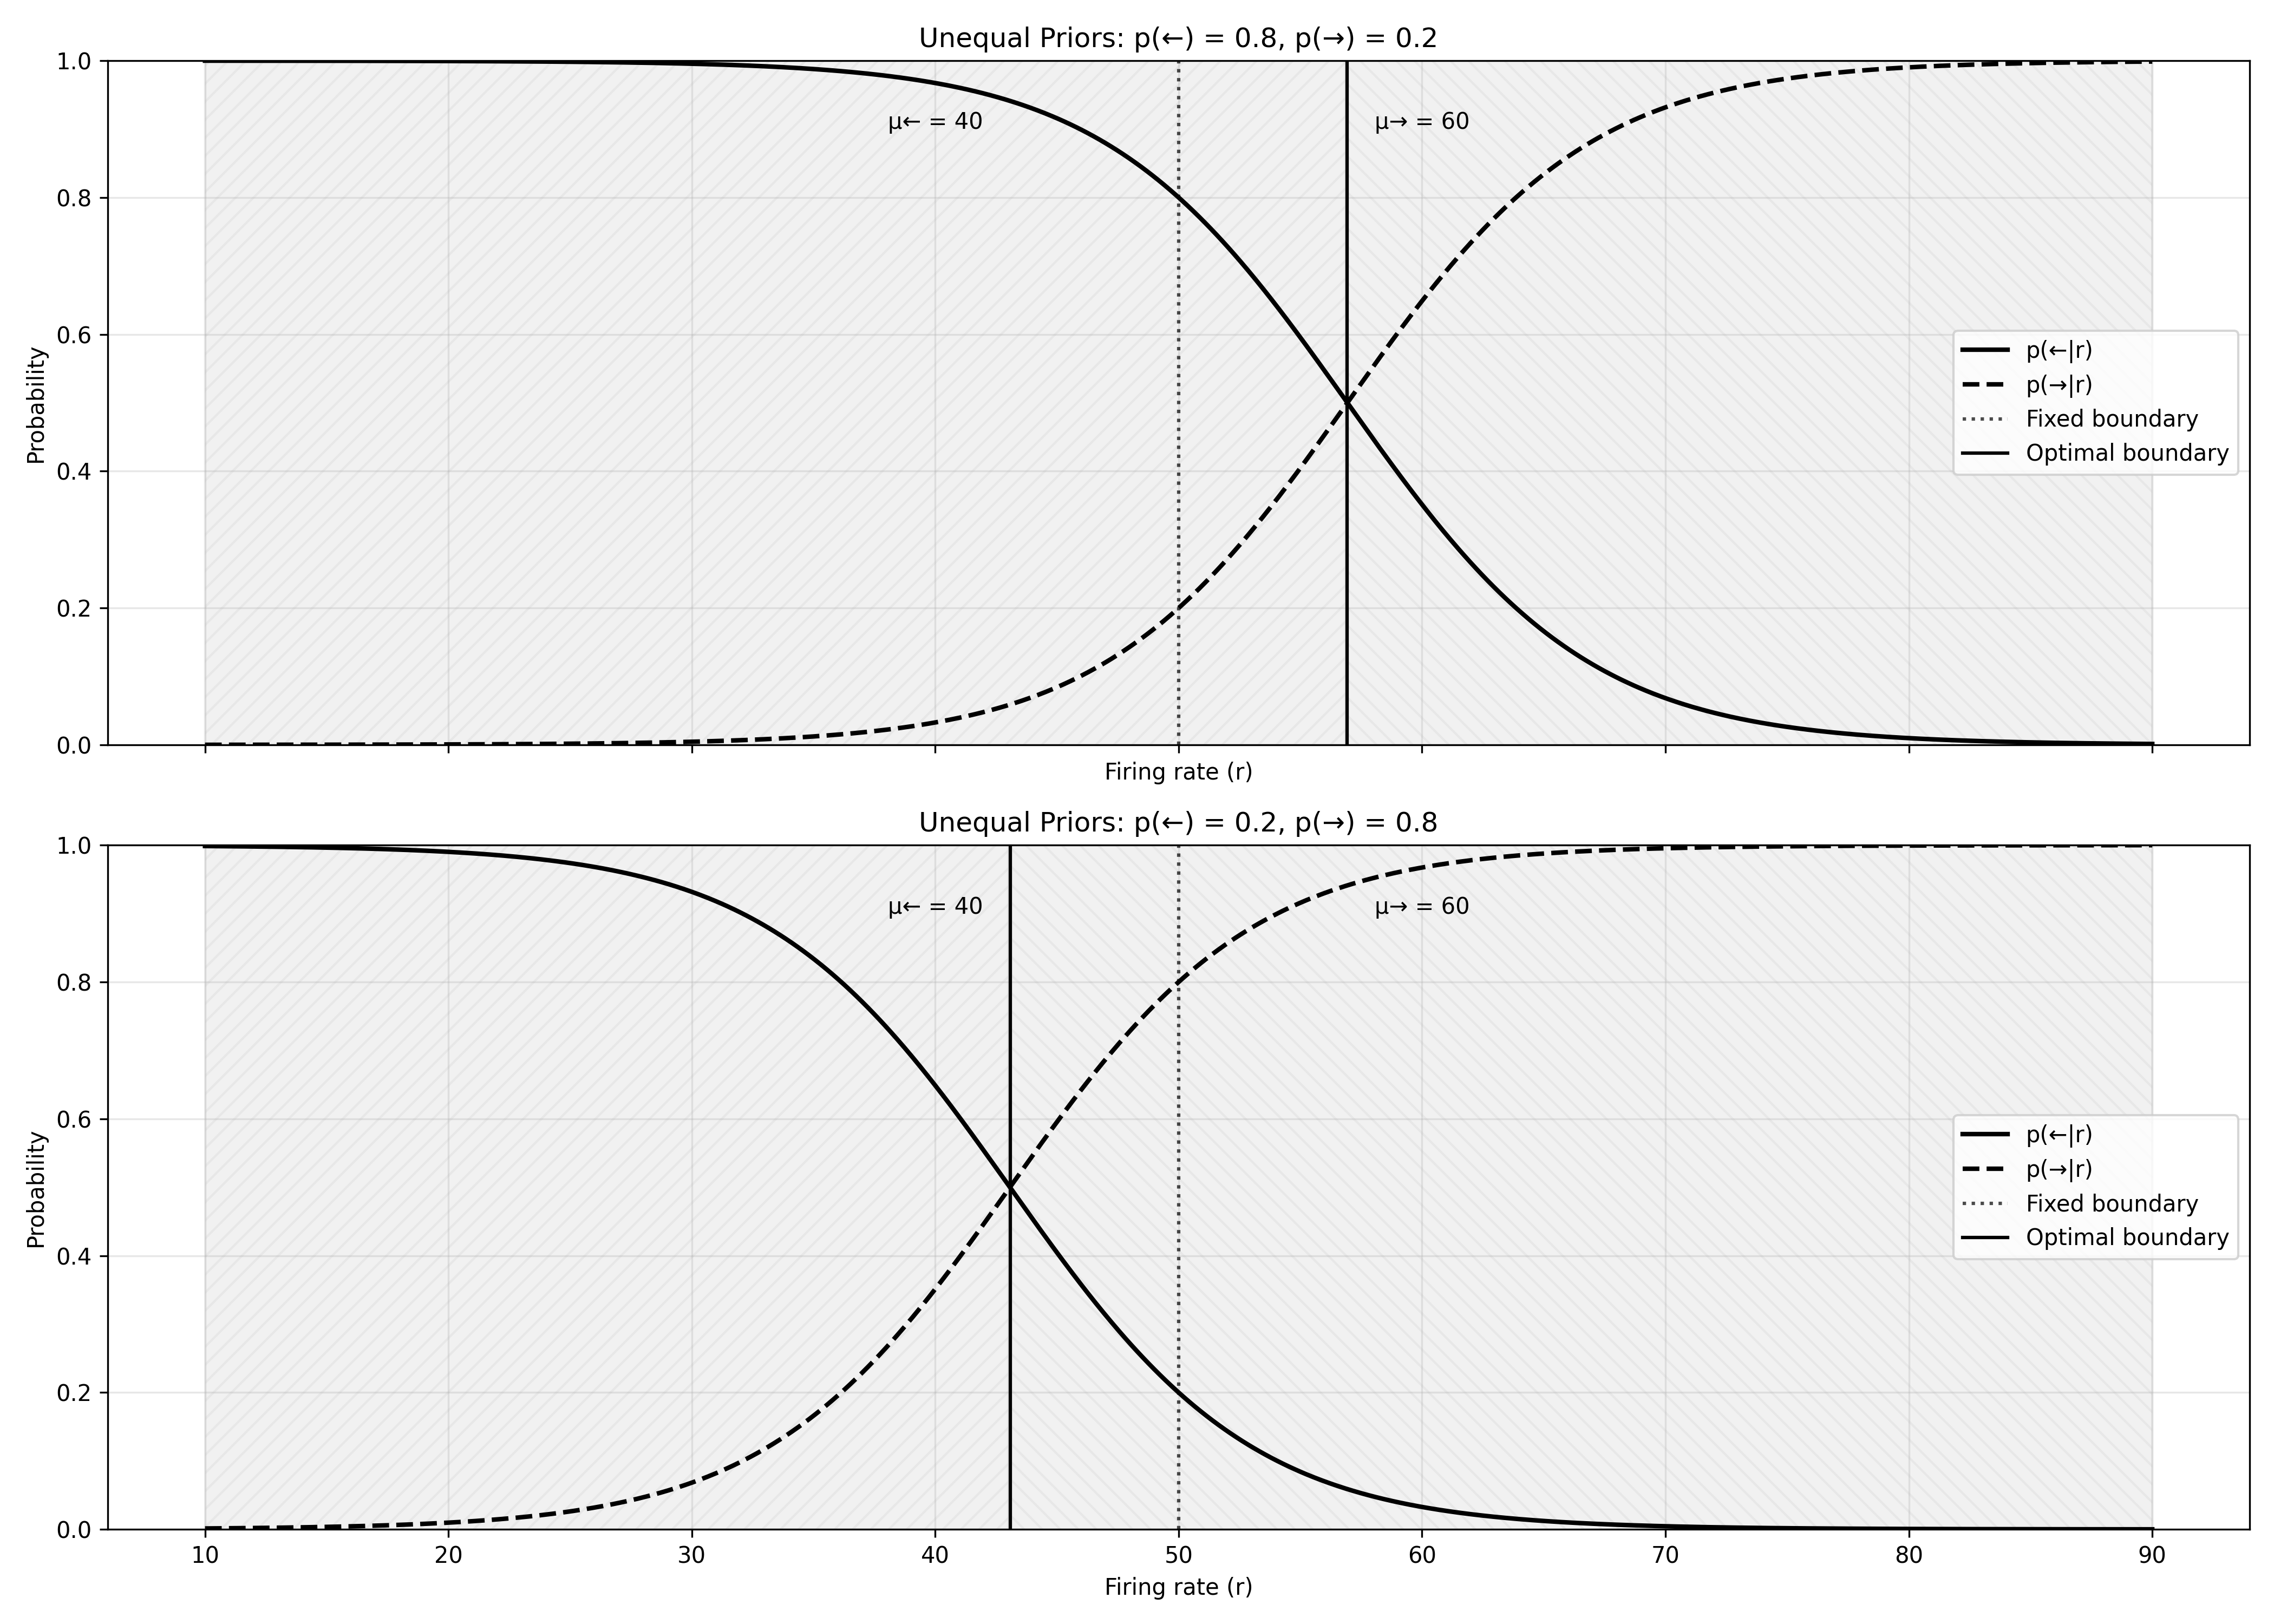
\includegraphics[width=0.8\textwidth]{posterior_unequal_priors.png}
    \caption{Posterior probabilities with unequal priors. 
    Top: When $p(\leftarrow) = 0.8, p(\rightarrow) = 0.2$, the decision boundary shifts to the right, 
    favoring leftward motion decisions for a wider range of firing rates.
    Bottom: When $p(\leftarrow) = 0.2, p(\rightarrow) = 0.8$, the decision boundary shifts to the left,
    favoring rightward motion decisions. 
}
    \label{fig:bayes_unequal_priors}
\end{figure}


\subsection{Decision rule analysis}
The decision rule $r > \frac{1}{2}(\mu_\leftarrow + \mu_\rightarrow)$ corresponds to choosing the stimulus with the higher likelihood when priors are equal. This is equivalent to the point where the posteriors cross ($p(\leftarrow|r) = p(\rightarrow|r) = 0.5$) under equal priors.

When prior probabilities are unequal, the fixed decision threshold no longer aligns with the point where the posterior probabilities intersect. As a result, the decision rule ignores prior information about stimulus frequency, potentially leading to suboptimal performance and increased error rates.

By using a simple threshold instead of the full posterior, we lose the ability to properly account for prior probabilities, the ability to express confidence in our decisions, the  probabilistic information provided by the posterior and the flexibility to optimize different decision criteria (e.g., minimizing total error vs. avoiding false alarms)

\section{Linear discriminant analysis}

\subsection{Computing the log-likelihood ratio}
The log-likelihood ratio is:
\begin{align}
l(r) &= \log\frac{p(r|\leftarrow)}{p(r|\rightarrow)}
\end{align}

Substituting the multivariate Gaussian distributions:
\begin{align}
l(r) &= \log\frac{\frac{1}{(2\pi)^{N/2}\sqrt{\det C}} \exp\left(-\frac{1}{2}(r - \mu_\leftarrow)^T C^{-1} (r - \mu_\leftarrow)\right)}{\frac{1}{(2\pi)^{N/2}\sqrt{\det C}} \exp\left(-\frac{1}{2}(r - \mu_\rightarrow)^T C^{-1} (r - \mu_\rightarrow)\right)} \\
&= \log\exp\left(-\frac{1}{2}(r - \mu_\leftarrow)^T C^{-1} (r - \mu_\leftarrow) + \frac{1}{2}(r - \mu_\rightarrow)^T C^{-1} (r - \mu_\rightarrow)\right) \\
&= -\frac{1}{2}(r - \mu_\leftarrow)^T C^{-1} (r - \mu_\leftarrow) + \frac{1}{2}(r - \mu_\rightarrow)^T C^{-1} (r - \mu_\rightarrow)
\end{align}

Expanding the quadratic forms:
\begin{align}
l(r) &= -\frac{1}{2}\left[r^T C^{-1} r - r^T C^{-1} \mu_\leftarrow - \mu_\leftarrow^T C^{-1} r + \mu_\leftarrow^T C^{-1} \mu_\leftarrow\right] \\
&\quad + \frac{1}{2}\left[r^T C^{-1} r - r^T C^{-1} \mu_\rightarrow - \mu_\rightarrow^T C^{-1} r + \mu_\rightarrow^T C^{-1} \mu_\rightarrow\right]
\end{align}

The $r^T C^{-1} r$ terms cancel out, and since $C$ is symmetric, $r^T C^{-1} \mu = \mu^T C^{-1} r$:
\begin{align}
l(r) &= \frac{1}{2}\left[2r^T C^{-1} (\mu_\leftarrow - \mu_\rightarrow) - \mu_\leftarrow^T C^{-1} \mu_\leftarrow + \mu_\rightarrow^T C^{-1} \mu_\rightarrow\right] \\
&= r^T C^{-1} (\mu_\leftarrow - \mu_\rightarrow) - \frac{1}{2}\left[\mu_\leftarrow^T C^{-1} \mu_\leftarrow - \mu_\rightarrow^T C^{-1} \mu_\rightarrow\right] = 0
\end{align}

This is a linear equation in $r$, which can be written as:
\begin{align}
r^T w + b = 0
\end{align}

where:
\begin{align}
w &= C^{-1}(\mu_\leftarrow - \mu_\rightarrow) \\
b &= -\frac{1}{2}\left[\mu_\leftarrow^T C^{-1} \mu_\leftarrow - \mu_\rightarrow^T C^{-1} \mu_\rightarrow\right]
\end{align}

This defines a hyperplane (linear) in the $N$-dimensional firing rate space. This hyperplane separates the regions where $l(r) > 0$ (classified as leftward motion) from regions where $l(r) < 0$ (classified as rightward motion).

\subsection{Decision boundary with uncorrelated neurons}
With $p(\leftarrow) = p(\rightarrow) = 1/2$ and a diagonal covariance matrix $C = \text{diag}(\sigma_1^2, \sigma_2^2)$, we have:
\begin{align}
C^{-1} = \text{diag}\left(\frac{1}{\sigma_1^2}, \frac{1}{\sigma_2^2}\right)
\end{align}

Let's denote $\mu_\leftarrow = [\mu_{\leftarrow,1}, \mu_{\leftarrow,2}]^T$ and $\mu_\rightarrow = [\mu_{\rightarrow,1}, \mu_{\rightarrow,2}]^T$.

The decision boundary equation becomes:
\begin{align}
&\left[\begin{array}{cc} r_1 & r_2 \end{array}\right] \left[\begin{array}{cc} \frac{1}{\sigma_1^2} & 0 \\ 0 & \frac{1}{\sigma_2^2} \end{array}\right] \left[\begin{array}{c} \mu_{\leftarrow,1} - \mu_{\rightarrow,1} \\ \mu_{\leftarrow,2} - \mu_{\rightarrow,2} \end{array}\right] \\
&- \frac{1}{2}\left[ \left[\begin{array}{cc} \mu_{\leftarrow,1} & \mu_{\leftarrow,2} \end{array}\right] \left[\begin{array}{cc} \frac{1}{\sigma_1^2} & 0 \\ 0 & \frac{1}{\sigma_2^2} \end{array}\right] \left[\begin{array}{c} \mu_{\leftarrow,1} \\ \mu_{\leftarrow,2} \end{array}\right] - \left[\begin{array}{cc} \mu_{\rightarrow,1} & \mu_{\rightarrow,2} \end{array}\right] \left[\begin{array}{cc} \frac{1}{\sigma_1^2} & 0 \\ 0 & \frac{1}{\sigma_2^2} \end{array}\right] \left[\begin{array}{c} \mu_{\rightarrow,1} \\ \mu_{\rightarrow,2} \end{array}\right] \right] = 0
\end{align}

Simplifying:
\begin{align}
&\frac{r_1}{\sigma_1^2}(\mu_{\leftarrow,1} - \mu_{\rightarrow,1}) + \frac{r_2}{\sigma_2^2}(\mu_{\leftarrow,2} - \mu_{\rightarrow,2}) \\
&- \frac{1}{2}\left[ \frac{\mu_{\leftarrow,1}^2}{\sigma_1^2} + \frac{\mu_{\leftarrow,2}^2}{\sigma_2^2} - \frac{\mu_{\rightarrow,1}^2}{\sigma_1^2} - \frac{\mu_{\rightarrow,2}^2}{\sigma_2^2} \right] = 0
\end{align}

This is a straight line in the $(r_1, r_2)$ plane, which can be written in the form:
\begin{align}
a r_1 + b r_2 + c = 0
\end{align}

where:
\begin{align}
a &= \frac{\mu_{\leftarrow,1} - \mu_{\rightarrow,1}}{\sigma_1^2} \\
b &= \frac{\mu_{\leftarrow,2} - \mu_{\rightarrow,2}}{\sigma_2^2} \\
c &= -\frac{1}{2}\left[ \frac{\mu_{\leftarrow,1}^2 - \mu_{\rightarrow,1}^2}{\sigma_1^2} + \frac{\mu_{\leftarrow,2}^2 - \mu_{\rightarrow,2}^2}{\sigma_2^2} \right]
\end{align}

The slope of this line is $-\frac{a}{b} = -\frac{\sigma_2^2(\mu_{\leftarrow,1} - \mu_{\rightarrow,1})}{\sigma_1^2(\mu_{\leftarrow,2} - \mu_{\rightarrow,2})}$.

This boundary optimally separates the two Gaussian distributions in the firing rate space. The orientation of the line depends on the difference in means and the variances of the two neurons (Fig 3).

\begin{figure}[h]
    \centering
    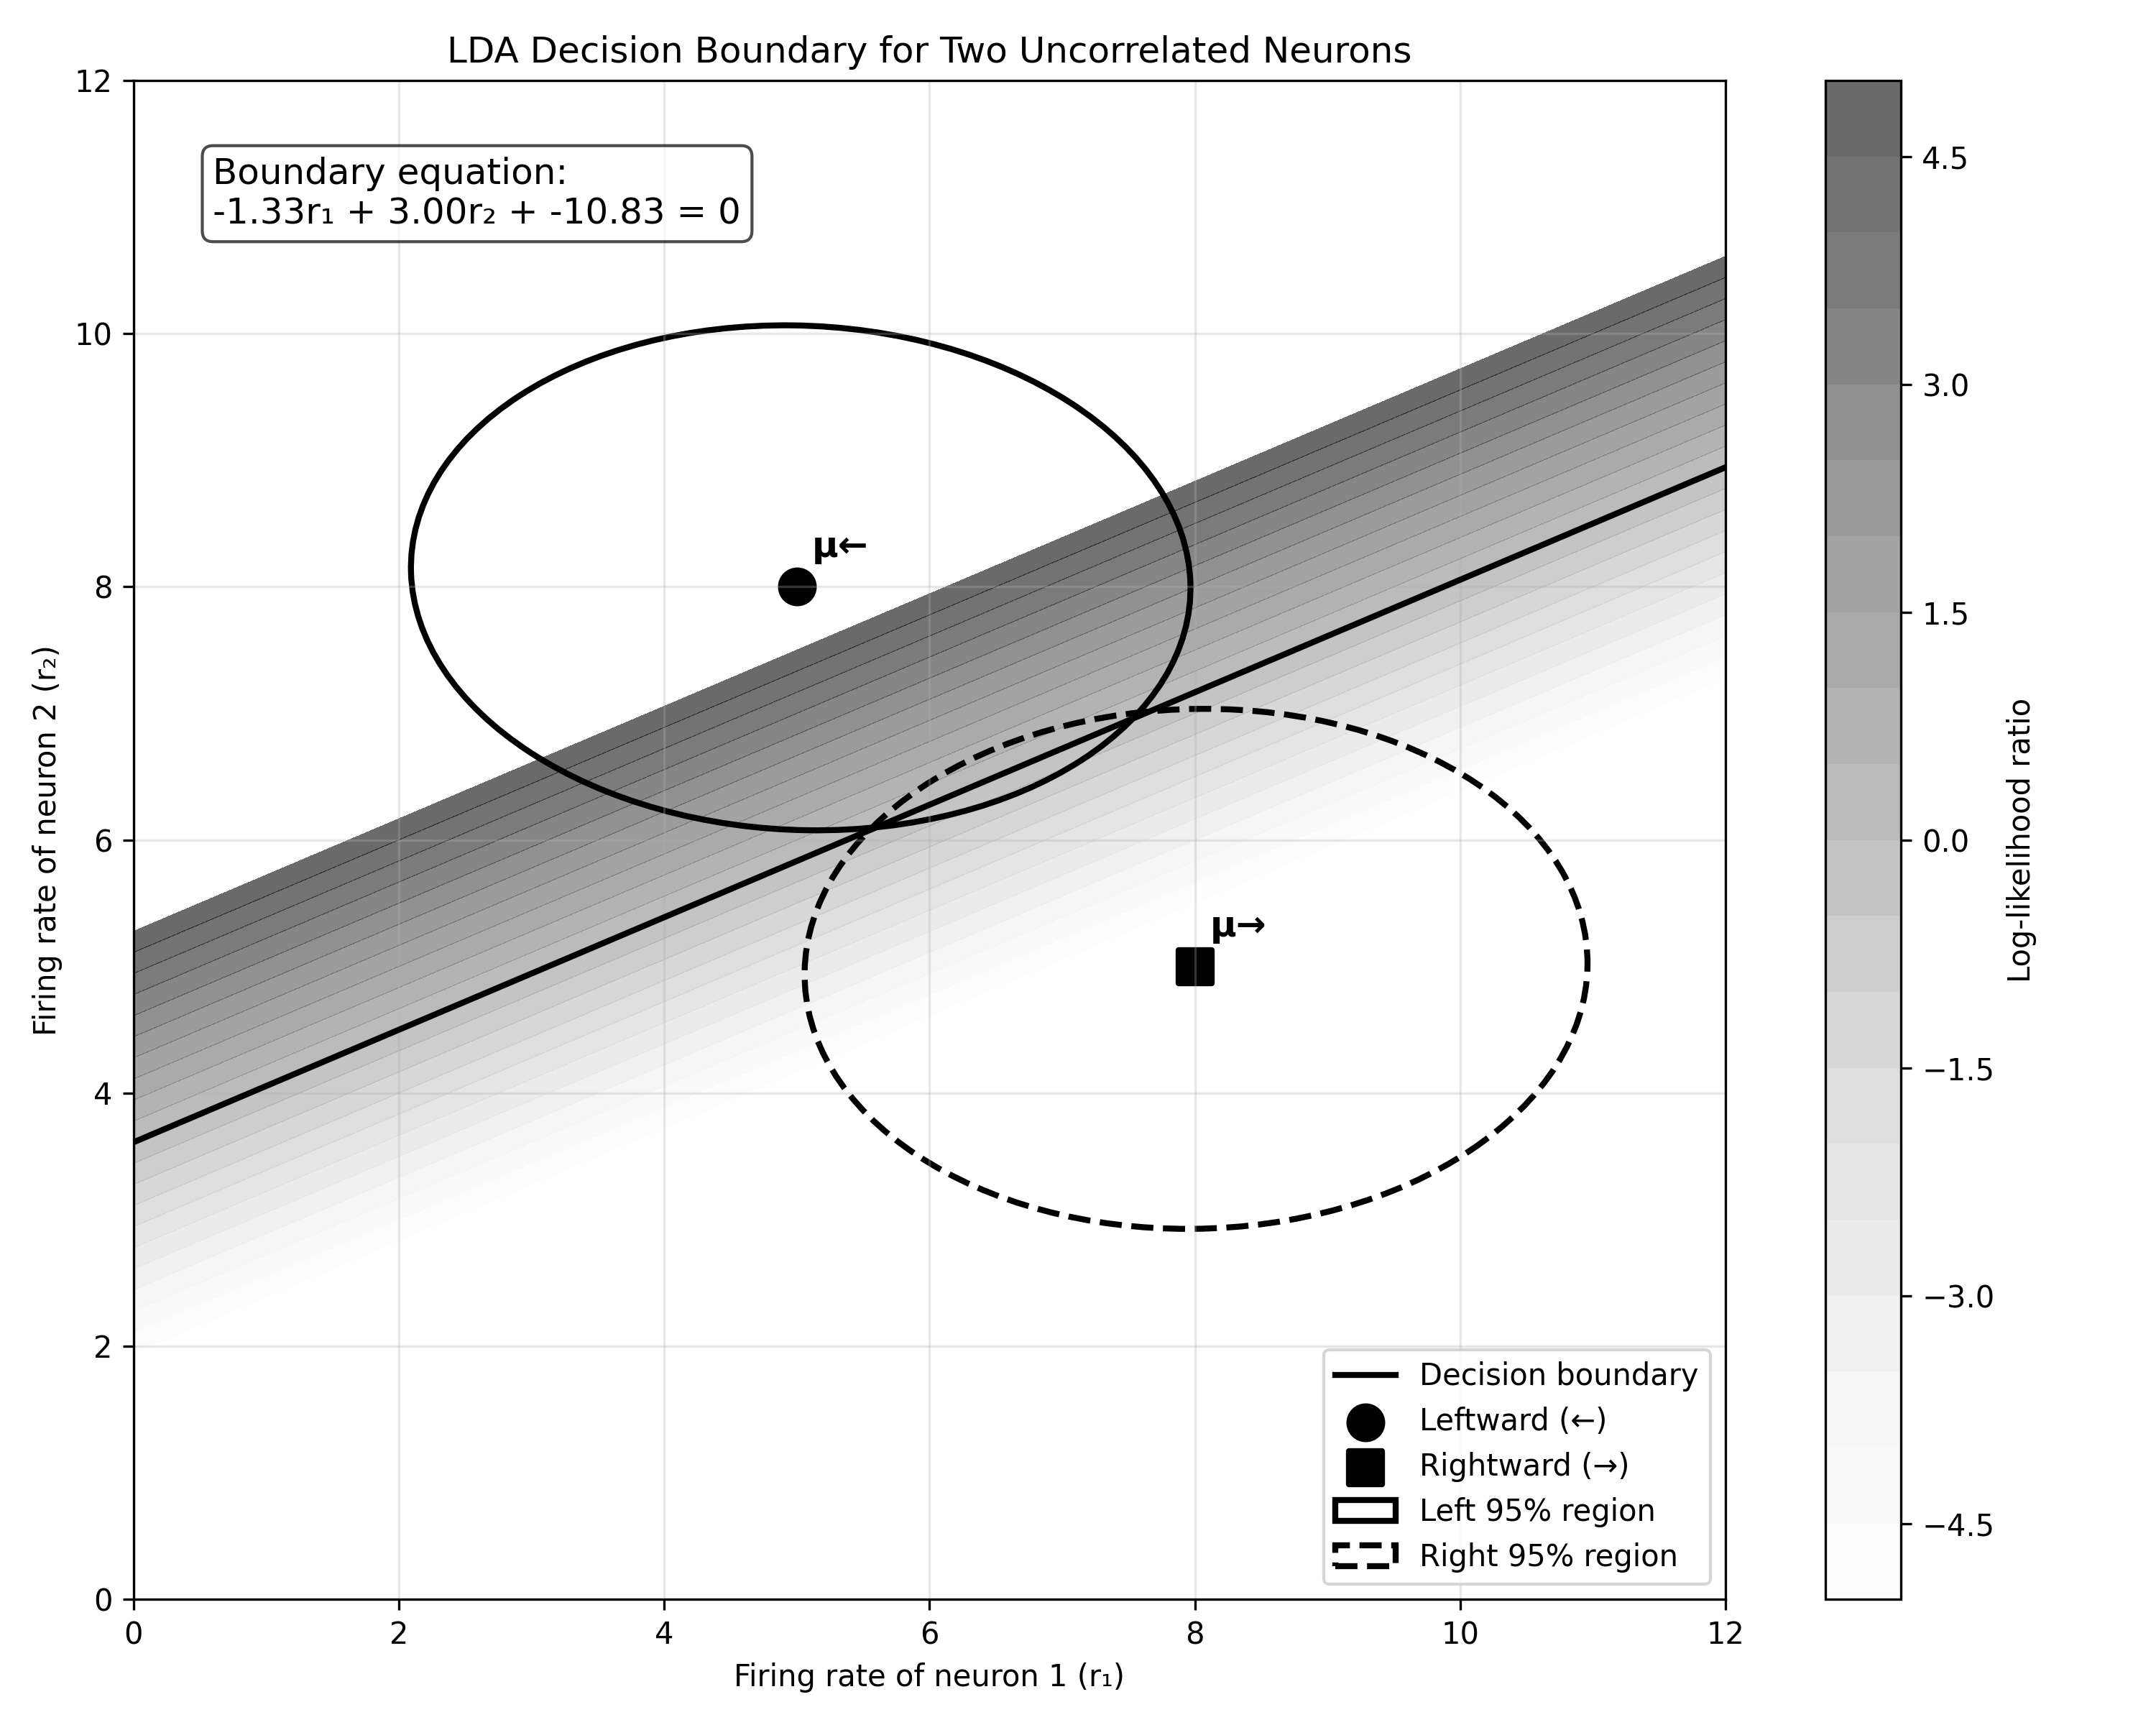
\includegraphics[width=0.8\textwidth]{lda_decision_boundary.png}
    \caption{This figure illustrates the LDA decision boundary for a 2D case with two uncorrelated neurons responding to different motion directions. The grayscale contour plot represents the log-likelihood ratio between leftward and rightward motion. The parameters are: mean firing rates for leftward motion $\mu_{\leftarrow} = [5, 8]$, mean firing rates for rightward motion $\mu_{\rightarrow} = [8, 5]$, with standard deviations $\sigma_1 = 1.5$ and $\sigma_2 = 1.0$. The solid black line represents the decision boundary, which optimally separates the two motion categories. The 95\% confidence regions for each motion direction are shown as ellipses. The decision boundary is defined by a linear equation based on the firing rates of both neurons, demonstrating how the neurons could optimally decode motion direction from neural activity patterns.}
    \label{fig:lda_boundary}
\end{figure}


\end{document}